\documentclass[10pt,a4j,dvipdfmx]{jsarticle}
\usepackage[utf8]{inputenc}
\usepackage[dvipdfmx]{graphicx}
\usepackage[usenames,dvipdfmx]{color}
\usepackage{amsmath}
\usepackage{bm}
\usepackage[left=19.05mm, right=19.05mm, top=25.40mm, bottom=25.40mm]{geometry}
\usepackage{tikz}
\usepackage{circuitikz}
\usepackage{siunitx}
\usepackage{listings}
\usepackage{float}
\usepackage{hyperref}
\usepackage{enumitem}

\lstset{%
  language={C},
  basicstyle={\small},%
  identifierstyle={\small},%
  commentstyle={\small\itshape},%
  keywordstyle={\small\bfseries},%
  ndkeywordstyle={\small},%
  stringstyle={\small\ttfamily},
  frame={tb},
  breaklines=true,
  columns=[l]{fullflexible},%
  numbers=left,%
  xrightmargin=0zw,%
  xleftmargin=3zw,%
  numberstyle={\scriptsize},%
  stepnumber=1,
  numbersep=1zw,%
  lineskip=-0.5ex%
}

\usepackage{fouriernc}
\usepackage[scaled]{helvet}
\usepackage[T1]{fontenc}
\renewcommand{\ttdefault}{fvm}

\let\oldthefootnote\thefootnote
\def\thefootnote{{\color{Magenta}\oldthefootnote}}

\newcommand{\enhance}[1]{{\gtfamily\sffamily#1}}
\makeatletter
\def\@jikkenname{}
\def\@jikkennum{}
\def\@reportname{}
\def\@studentnumber{}
\def\@studentname{}
\def\@studentdepartment{}
\def\@friendnames{}
\def\@groupnumber{}
\newcommand{\jikkenset}[2]{\def\@jikkennum{#1}\def\@jikkenname{#2}}
\newcommand{\studentset}[3]{\def\@studentnumber{#1}\def\@studentname{#2}\def\@studentdepartment{#3}}
\newcommand{\reportnameset}[1]{\def\@reportname{#1}}
\newcommand{\friendname}[1]{\def\@friendnames{#1}}
\newcommand{\groupnumber}[1]{\def\@groupnumber{#1}}
\renewcommand{\maketitle}{
\noindent{\color{RoyalPurple}\hrule height 1pt \hfill}
\vspace{5pt}
\begin{center}
\enhance{{\Large{電気電子情報第一(前期)実験}}}\\[7pt]
\enhance{{\Huge\textbf{\@jikkennum{}. \@jikkenname}}}\\[5pt]
\enhance{{\LARGE{\@reportname}}}\\[15pt]
\@studentnumber\ \ \ \@studentname{}(\@studentdepartment{})\\[1pt]
共同実験者: \@friendnames(第\@groupnumber{}班)\\[1pt]
\today
\end{center}
\vspace{-10pt}
\noindent{\color{RoyalPurple}\hrule height 1pt \hfill}
}
\makeatother
\jikkenset{A1}{半導体と電子回路の基礎}
\reportnameset{考察レポート}
\studentset{03-160441}{土屋潤一郎}{工学部 電子情報工学科}
\friendname{井上友貴、田中大幹、坂口達彦}
\groupnumber{28}

\makeatletter
\let\@oldsec\section
\let\@oldsubsec\subsection
\renewcommand{\section}[1]{\@oldsec{#1}\vspace{-5pt}{\color{TealBlue}\hrule height 0.6pt \hfill}\par}
\renewcommand{\thesection}{\arabic{section}.}
\renewcommand{\subsection}[1]{\vspace{-7pt}\@oldsubsec{#1}}
\makeatother

\begin{document}
\maketitle

\section{実験の概要}
\begin{description}
 \item[第1日]pn接合ダイオードの電流・電圧特性の計測
 \item[第2日]JunctionFETの電流・電圧特性の計測
 \item[第3日]ソース接地増幅回路の動作点決定と入出力特性の計測
 \item[第4日]ソース接地増幅回路の周波数特性の計測
\end{description}
\section{考察}
\subsection{pn接合ダイオードの電流電圧特性と電圧計・電流計の内部抵抗}
\subsubsection{電流計の内部抵抗}

\begin{figure}[H]
  \centering
\begin{circuitikz}
\draw (0,1) to [short,i>=$I_{measured}$, o-] (1,1) to [esource, l =$r$, -] (4,1);
\draw (1,1) to [short, *-*] (1,-1.2) to [short, -*] (1,-2.2) to [short, -*] (1,-3.2) to [short, -] (1,-4.2);
\draw (1,-0.2) to [open, -o] (4,-0.2);
\draw (1,-1.2) to [R, l =$R_1$, -o] (4,-1.2);
\draw (1,-2.2) to [R, l =$R_2$, -o] (4,-2.2);
\draw (1,-3.2) to [R, l =$R_3$, -o] (4,-3.2);
\draw (1,-4.2) to [R, l =$R_4$, -o] (4,-4.2);
\draw (4,1) to [short, -*] (6,1) to [short, -o] (6.5,1);
\draw (6,1) to [short, -] (6,-2.2);
\draw (6, -2.2) to [short, -o] (5.5,-2.2);
\draw (5.5,-2.2) to [short, -] (4,-0.2);
\end{circuitikz}  
\caption{電流計内部の指示計器と分流器}
\end{figure}

電流計では分流器として用いる抵抗を切り替えられるようにして、測定レンジの切り替えを実現している(図1)。
従って考えなければならない内部抵抗は、指示計器が持つ内部抵抗r[\si{\ohm}]に加え、分流器の持つ内部抵抗R[\si{\ohm}]である。
電流計ではこの2つが並列になっているから、テスタで測定される内部抵抗は$\left(\frac{1}{r}+\frac{1}{R}\right)^{-1}$[\si{\ohm}]で、測定レンジの最も小さなものでは$R=\infty$(すなわち、測定値がそのままrで、このレンジを$i_{max}$とする)と考えた時のRの値と、そこから$I_{max} = \left(\frac{r}{R} + 1\right)i_{max}$で導出される計算上の測定レンジ、逆に公称の測定レンジから推測される$R_{T}$と$\left(\frac{1}{r}+\frac{1}{R_{T}}\right)^{-1}$とは以下の表1及び表2の通りであった。

\begin{table}[htb]
  \centering
    \caption{内部抵抗(\si{\milli\ampere}レンジの電流計)}
    \begin{tabular}{|l||c|r|r||r|c|} \hline
      レンジ[\si{\milli\ampere}] & $\left(\frac{1}{r}+\frac{1}{R}\right)^{-1}$[\si{\ohm}] & R[\si{\ohm}] & Imax[\si{\milli\ampere}] & $R_{T}$\si{\ohm} & $\left(\frac{1}{r}+\frac{1}{R_{T}}\right)^{-1}$\si{\ohm} \\ \hline \hline
      10 & 4.3 & $\infty$ & 10 & 4.3 & 4.3\\
      30 & 1.5 & 2.30 & 28.7 & 2.15 & 1.43\\
      100 & 0.5 & 0.566 & 86 & 0.478 & 0.43\\ 
      300 & 0.2 & 0.210 & 215 & 0.148 & 0.143\\ 
      1000 & 0.1 & 0.102 & 430 & 0.0434 & 0.043\\ 
      \hline
    \end{tabular}
\end{table}

\begin{table}[htb]
  \centering
    \caption{内部抵抗測定値(\si{\micro\ampere}レンジの電流計)}
    \begin{tabular}{|l||c|r|r||r|c|} \hline
      レンジ[\si{\micro\ampere}] & $\left(\frac{1}{r}+\frac{1}{R}\right)^{-1}$[\si{\ohm}] & R[\si{\ohm}] & Imax[\si{\micro\ampere}] & $R_{T}$[\si{\ohm}] & $\left(\frac{1}{r}+\frac{1}{R_{T}}\right)^{-1}$[\si{\ohm}] \\ \hline \hline
      30 & $4.7\times10^3$ & $\infty$ & 30 & $4.7\times10^3$ & 4700\\
      100 & $6.71\times10^3$ & -15690 & 21.0 & $2.01\times10^3$ & 1410 \\
      300 & $2.744\times10^3$ & 6593 & 51.4 & $5.222\times10^2$ & 470\\
      1000 & $0.877\times10^3$ & 1078 & 161 & $1.45\times10^2$ & 141\\
      3000 & 297.4 & 317.4 & 474 & $4.747\times10^1$ & 47 \\ \hline
    \end{tabular}
\end{table}

\subsubsection{電圧計の内部抵抗}
\begin{figure}[H]
  \centering
\begin{circuitikz}
\draw (0,0) to [short,-o] (0,1);
\draw (7.5,0) to [short,-o] (7.5,1);
\draw (0,1) to [open, v^>=$V_{measured}$] (7.5,1);
\draw (0,0) to [short,-] (4,0) to [short,-] (5.5,0) to [esource, l =$r$, -] (7.5,0);
\draw (1,0) to [short, *-*] (1,-1.2) to [short, -*] (1,-2.2) to [short, -*] (1,-3.2) to [short, -] (1,-4.2);
\draw (1,-1.2) to [R, l =$R_1$, -o] (4,-1.2);
\draw (1,-2.2) to [R, l =$R_2$, -o] (4,-2.2);
\draw (1,-3.2) to [R, l =$R_3$, -o] (4,-3.2);
\draw (1,-4.2) to [R, l =$R_4$, -o] (4,-4.2);
\draw (5.5,0) to [short, *-] (5.5,-2.2);
\draw (5.5,-2.2) to [short, -o] (5,-2.2);
\draw (5,-2.2) to [short, -o] (4,0);
\end{circuitikz}
\caption{電圧計内部の指示計器と倍率器}
\end{figure}

電圧計では倍率器として用いる抵抗を切り替えられるようにして、測定レンジの切り替えを実現している(図2)。
従って考えなければならない内部抵抗は、指示計器が持つ内部抵抗r[\si{\ohm}]に加え、倍率器の持つ内部抵抗R[\si{\ohm}]である。
電圧計ではこの2つが直列になっているから、テスタで測定される内部抵抗は$r+R$[\si{\ohm}]で、測定レンジの最も小さなものでは$R=0$(すなわち、測定値がそのままrで、このレンジを$v_{max}$とする)と考えた時のRの値と、そこから$V_{max} = \left(\frac{R}{r} + 1\right)v_{max}$で導出される計算上の測定レンジ、逆に公称の測定レンジから推測される$R_{T}$と$r+R_T$とは以下の表3の通りであった。

\begin{table}[htb]
  \centering
    \caption{内部抵抗(電圧計)}
    \begin{tabular}{|l||c|r|r||r|c|} \hline
      レンジ[\si{\volt}] & $r+R$[\si{\kilo\ohm}] & R[\si{\kilo\ohm}] & Vmax[\si{\volt}] & $R_{T}$[\si{\kilo\ohm}] & $r + R_T$[\si{\kilo\ohm}] \\ \hline \hline
      0.3 & 3.025 & 0 & 0.3 & 0 & 3.025 \\
      1 & 10.05 & 7.025 & 0.997 & 7.058 & 10.08\\
      3 & 30.12 & 27.10 & 2.99 & 27.23 & 30.25\\ 
      10 & 100.5 & 97.48 & 9.97 & 97.81 & 100.8\\ 
      30 & 301.6 & 298.6 & 29.9 & 299.5 & 302.5\\ 
      \hline
    \end{tabular}
\end{table}

\subsubsection{測定値の補正}
これら2.1.1節及び2.1.2節に従うならば、まず、読み取った値を、$I_{max}$や$V_{max}$の値と公称の測定レンジの比から補正し、その後で測定系の回路構造と内部抵抗を考慮した補正を行うべきであろう。

しかし、$V_{max}$と公称レンジの誤差が0.3$\sim$0.4\%である電圧計はともかく、電流計の$I_{max}$と公称レンジの誤差は\si{\milli\ampere}レンジで最大57\%、\si{\micro\ampere}レンジに至っては(最小レンジ以外では)80\%前後の値となる。
その上\SI{100}{\micro\ampere}レンジでは\SI{30}{\micro\ampere}レンジよりも大きな抵抗値を示しており、そこから導出される分流器の抵抗は負の値となってしまっている。

本来であれば表1$\sim$3を完成させるような計算を実験中に行い、すぐさま電流計を他のものに交換すべきであったが、
ダイオードの特性測定中には測定系の回路構造と内部抵抗を考慮した補正にだけ意識を取られ、幾度も内部抵抗を測定しなおして首を捻るばかりであった。

一応、次節以後のダイオードの測定に関する考察は、電流計の読み取った値の補正を、表1及び表2に従って行っている。

\subsubsection{ダイオードのVI特性(順バイアス時)}
\begin{figure}[H]
\centering
\begin{tabular}{cc}
\begin{minipage}{0.5\hsize}
\centering
\begin{circuitikz}
\draw (0,0) to [short,-] (0.5,0) to [ammeter,-] (3.5,0) to [short,-*] (4,0) to [short, -] (5,0);
\draw (0,-3) to [battery,-] (0,0);
\draw (0,-3) to [short, -] (5,-3);
\draw (4,0) to [voltmeter,*-*] (4,-3);
\draw (5,0) to [Do,-] (5,-3);
\end{circuitikz}
\caption{順バイアス時の測定系の模式図(a)}
\end{minipage}

\begin{minipage}{0.5\hsize}
\centering
\begin{circuitikz}
\draw (0,0) to [short,-*] (1,0)to [short,-] (1.5,0) to [ammeter,-] (4.5,0) to [short,-] (5,0);
\draw (0,-3) to [battery,-] (0,0);
\draw (0,-3) to [short, -] (5,-3);
\draw (1,0) to [voltmeter,*-*] (1,-3);
\draw (5,0) to [Do,-] (5,-3);
\end{circuitikz}
\caption{順バイアス時の測定系の模式図(b)}
\end{minipage}
\end{tabular}
\end{figure}
さて、前項までの考察によって判明した、用いた電流計が非常に不正確であったことも踏まえつつ、pn接合ダイオードの順バイアス時の測定結果の補正値と、理論値を図5に示す。
理論曲線(灰色)は$I=I_s\exp\left(\frac{qV}{kT}-1\right) $と測定結果を比較して$I_s$を決定したものである(但し、$T=300[\si{\kelvin}]$とした)。決定された逆方向飽和電流は$I_s = 7.69\times10^{-15}[\si{\ampere}]$である。

\begin{figure}[H]
  \centering
  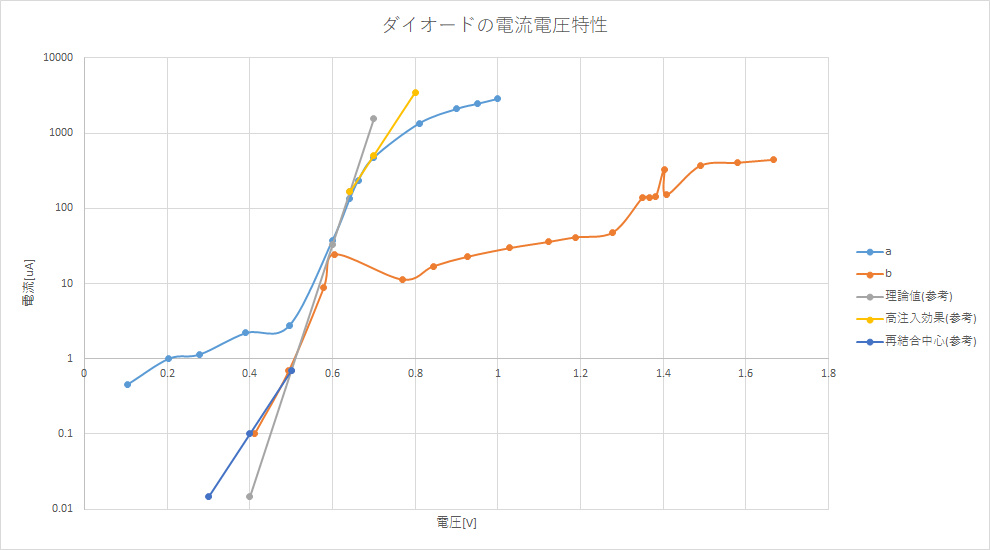
\includegraphics[width=15cm]{Diode.png}
  \caption{順バイアス時測定結果と予測される理論値}
\end{figure}

図5を見ると、\SI{0.6}{\volt}周辺を境にして、低電圧領域ではbが、高電圧領域ではaが、正しい測定結果を示していると考えるべきだろう。
従ってこの辺りが、補正を含めてのこれらの測定系の限界であると考えられる。
実際、図5の縦軸を線形にすると、そのグラフの傾きが\SI{0.6}{\volt}程度から急激に大きくなることがわかるが、これがコンダクタンスであるから、(補正の事を考えなければ)これが大きい領域では図3に示す回路aの測定方法を、小さい領域では図4に示す回路bの測定方法を用いるのが適している。

さて、0.5Vより低い電圧の領域では、(この範囲の有効な測定点は1つしか無いが、)理論値よりも大きな電流が流れている。これは空乏層に生成・再結合中心が存在し、過剰な電子とホールの再結合による余分な電流が流れるることが原因であろう。この電流は$\exp\left(\frac{qV}{2kT}\right)$に比例するが、実際にその理論値を取ってみた曲線が濃い青で示されるものである。

一方、おおよそ0.64$\sim$0.7\si{\volt}の範囲でも、電流が$\exp\left(\frac{qV}{2kT}\right)$に比例している(黄色い曲線)と考えられる。
これは、電子(の分布)に対して、ホールの分布が濃度勾配による拡散と電子とのクーロン力との吊り合いによって一定の分布に保たれるため電子の分布と一致せず、それによって存在する電界が高水準注入では無視できないことによる。

さらに高電圧な領域では、というよりは大電流の領域では、半導体そのものや配線などの抵抗による電圧降下が大きくなり、接合部にかかる電圧が見かけよりも小さくなっていく抵抗性領域に入ったと考えられる。

\subsubsection{ダイオードのVI特性(逆バイアス時)}
理想的なダイオードは、逆バイアスを掛ければ当然電流は0である。
今回の実験では図3と図4のダイオードを逆向きにした回路で計測したが、bでは電流計の針が触れなかった。
一方、aでは針が触れたが、これを補正したものが図6である。
\begin{figure}[H]
  \centering
  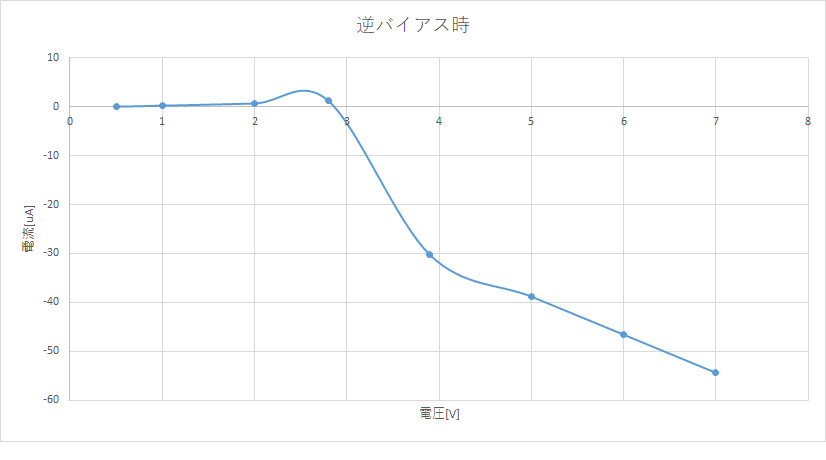
\includegraphics[width=15cm]{gyaku.png}
  \caption{逆バイアス時測定結果}
\end{figure}
使用した素子のデータシートによると、逆方向電流に当たる遮断電流$I_{GSS}$は最大で\SI{1.0}{\nano\ampere}であるから測定に用いた\si{\micro\ampere}レンジの電流計では測定不能であろうし、降伏電圧は\SI{-50}{\volt}なので今回の測定範囲にはない。
一方で、得られた電流のオーダーは最大でも$10^1$[\si{\micro\ampere}]の範囲である。
従って測定された電流は電圧計側に流れる電流で、補正の結果得られた値はノイズであると考えられる。

\subsection{JFETを用いたソース接地増幅回路の増幅率の周波数特性}

\begin{figure}[H]
\centering
\begin{circuitikz}
\draw (0,0) node[njfet](njfet) at(0,0){};
\draw (0,-0.27) -- (-3,-0.27);
\draw (-3,-0.27) -- (-3,-0.8)to [R, l = $R_G$] (-3,-3) node[ground]{};
\draw (-3,-0.27) to [C, l = $C_C$, *-o] (-5,-0.27) node[anchor=east]{$v_i$};
\draw (0,-0.8) to [R, l = $R_S$, *-] (0,-3) node[ground]{};
\draw (0,-0.8) -- (1.5,-0.8) to [C, l = $C_S$, *-] (1.5,-3) node[ground]{};
\draw (njfet.D) to [R, l = $R_L$, *-] (0,3) -- (2,3) node[anchor=west]{$V_0$};
\draw (njfet.D) to [short,-o] (2,0.77) node[anchor=west]{$v_o$};
\end{circuitikz}
\caption{ソース接地増幅回路}
\end{figure}

図7のようなソース接地増幅回路で、オシロスコープを用いた電圧増幅率の周波数特性を測定した。

回路の設計にあたってはまず、動作点を決定するために負荷抵抗$R_L$[\si{\ohm}]と$V_0$[\si{\volt}]を決め、その条件での$V_{GS}V_{DS}$特性を眺めながら動作点を決定し、その周辺でのトランジスタの相互コンダクタンスを求めた。
これは前日までの実験の結果から、$R_L=10[\si{\kilo\ohm}]$、$V_0=30[\si{\volt}]$を採用し、動作点を\SI{1.2}{\volt}とした。
用いる相互コンダクタンス$g_m\si{\siemens}$として$V_{GS}I_{D}$特性の傾きを知るため、\SI{1.2}{\volt}とその前後3点の測定点を使用した。
その結果$g_m = -1.97\times10^{-3}[\si{\siemens}]$であった。

さて、ゲートソース間電圧は、ドレイン電流の直流成分が抵抗$R_S$を流れることによって動作点電圧となるわけだから、$V_{GS}$$I_{D}$特性から$R_S$の値を決定しなければならない。
この$R_S$の値は計算上\SI{834}{\ohm}であったが、実際には素子の組み合わせと精度の問題から\SI{830}{\ohm}とした。
この値を用いて$V_{GS}$$I_{D}$特性と同じグラフに負荷直線を引き直したものが、図8である。
交点がおおむね\SI{1.2}{\volt}にあることが確認できる。

\begin{figure}[H]
  \centering
  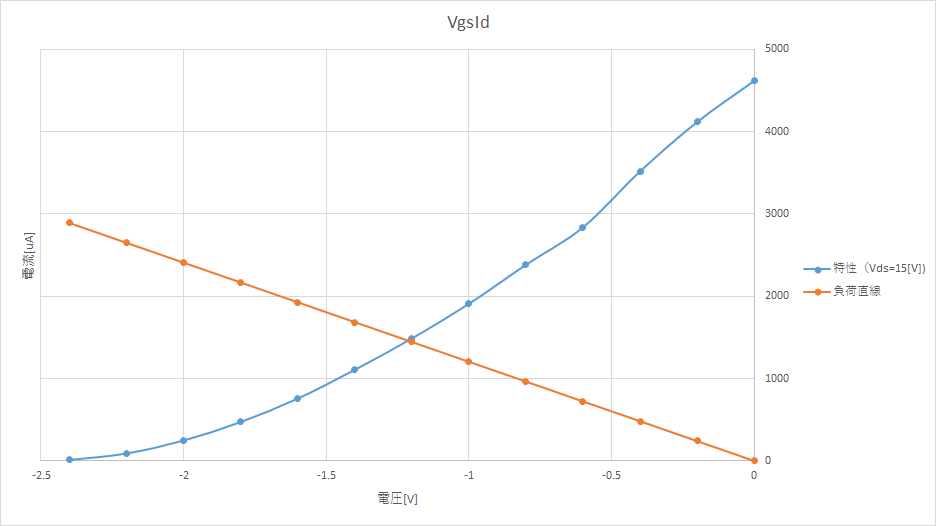
\includegraphics[width=8cm]{VgsId.png}
  \caption{ゲートソース間電圧・ドレイン電流特性と負荷直線}
\end{figure}
\subsubsection{中域周波数帯での電圧増幅率}
さて、中域の周波数では、電圧増幅率$A_v$は$A_v=-g_m R_L$となる。
これは計算上19.725で、これを利得に直すと\SI{25.90}{\decibel}である。

\begin{figure}[H]
  \centering
  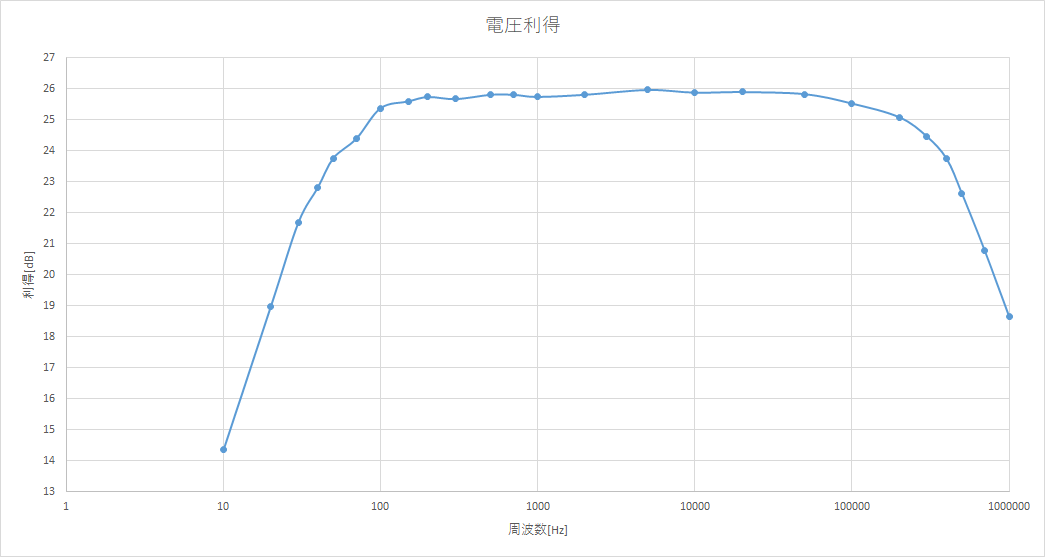
\includegraphics[width=15cm]{Gain.png}
  \caption{電圧利得の周波数特性}
\end{figure}

測定結果(図9)を見ると、平坦な領域の測定値は25.60$\sim$25.96\si{\decibel}に集まっているので、中域周波数の増幅率に関しては誤差なく設計できたといえるだろう。
\subsubsection{遮断周波数}
遮断周波数についても計算を行う。
理論上の値は、

\begin{align}
f_1 &= \frac{1}{2\pi C_C R_G} \\
f_2 &= \frac{1}{2\pi C_D R_L}
\end{align}

$R_G=100[\si{\kilo\ohm}]$の下で$f_1$が\SI{50}{\hertz}程度の値を取るように、$C_C = 0.033[\si{\micro\farad}]$とした。
従って、設計上の$f_1$は\SI{48.2}{\hertz}である。
測定結果(図9)を見ると、\SI{50}{\hertz}のとき\SI{23.8}{\decibel}であるから、中域周波数の利得から約\SI{-3}{\decibel}下がっているといえる。

もう一方の遮断周波数$f_2$[\si{\hertz}]から、ドレインの漂遊容量$C_D$[\si{\farad}]を逆算できる。
測定結果(図9)を見ると、$f_2 = 3.8\times10^4[\si{\hertz}]$程度だから、$C_D = 4.2\times10^2[\si{\pico\farad}]$である。

\section{参考資料}
\begin{enumerate}
\item 東京大学工学部電子情報工学科・電気電子工学科(2016)『電気電子情報第一(前期)実験テキスト』
\item 廣瀬明(2015)『電気電子計測[第2版]』数理工学社
\item 柴田直(2014)『半導体デバイス入門』数理工学社
\end{enumerate}

\end{document}
